%%%%%%%%%%%%%%%%%%%%%%%%%%%%%%%%%%%%%%%%%%%%%%%%%%%%%%%%%%%%%%%
% Important : Ces sources sont prévues pour être compilées avec XeTeX.
% Testé avec Texlive 2012.
% Encodage du texte en UTF-8
% Auteur : François Chaix <francois.chaix@etu.univ-lyon1.fr>
% Vous pouvez faire ce que vous voulez avec ce document et ce code, je le place
% sous la licence CC0 (https://creativecommons.org/publicdomain/zero/1.0/)
%%%%%%%%%%%%%%%%%%%%%%%%%%%%%%%%%%%%%%%%%%%%%%%%%%%%%%%%%%%%%%%

\documentclass[a4paper, 12pt, linktocpage=true, oneside]{memoir}
%\renewcommand{{\baselinestretch}}{1.5}
\renewcommand{\baselinestretch}{1.5}
\usepackage{polyglossia}
	\setdefaultlanguage{french}

\usepackage{geometry}
\geometry{hmargin=2.5cm,vmargin=2.5cm}

% \setmainfont[Mapping=tex-text]{Linux Libertine}
\usepackage{libertine}
% \renewcommand{\familydefault}{\sfdefault} % Pour utiliser une fonte sans empâtements (sans serif) par défaut (biolinum avec le package libertine)
\usepackage{lipsum}
\usepackage[%
    hidelinks=true
    colorlinks=false
    pdfauthor={François Chaix},
    pdftitle={Rapport de stage M1 François Chaix},
    pdfsubject={Dynamique des éléments transposables chez l'endosymbionte Wolbachia},
    pdfkeywords={Wolbachia, Transposon-display, Drosophila, parasite, endoparasite, symbiose, Leptopilina heterotoma},
    pdfproducer={XeteX, avec le package hyperref},
    pdfcreator={Xelatex}]{hyperref}
%\usepackage[sorting=none, backend=biber, style=nature]{biblatex}
%\bibliography{bib}
\usepackage[style=aem, natbib=true, backend=biber]{biblatex}
\addbibresource{bib.bib}

%\usepackage[Bjornstrup]{fncychap} % Ça c'était pour quand j'utilisais la classe report
\chapterstyle{hangnum}

\newenvironment{encart} 
   {\begin{quote} \footnotesize \renewcommand{\baselinestretch}{0}} 
   {\normalsize \end{quote}} 

%\makeatletter
\def\clap#1{\hbox to 0pt{\hss #1\hss}}%
\def\ligne#1{%
\hbox to \hsize{%
\vbox{\centering #1}}}%
\def\haut#1#2#3{%
\hbox to \hsize{%
\rlap{\vtop{\raggedright #1}}%
\hss
\clap{\vtop{\centering #2}}%
\hss
\llap{\vtop{\raggedleft #3}}}}%
\def\bas#1#2#3{%
\hbox to \hsize{%
\rlap{\vbox{\raggedright #1}}%
\hss
\clap{\vbox{\centering #2}}%
\hss
\llap{\vbox{\raggedleft #3}}}}%
\def\maketitle{%
\thispagestyle{empty}\vbox to \vsize{%
\haut{}{\@blurb}{}
\vfill
\vspace{1cm}
\begin{flushleft}
%\usefont{OT1}{ptm}{m}{n}
\huge \@title
\end{flushleft}
\par
\hrule height 4pt
\par
\begin{flushright}
%\usefont{OT1}{phv}{m}{n}
\Large \@author
\par
\end{flushright}
\vspace{1cm}
\vfill
\vfill
\bas{}{\@location, le \@date}{}
}%
\cleardoublepage
}
\def\date#1{\def\@date{#1}}
\def\author#1{\def\@author{#1}}
\def\title#1{\def\@title{#1}}
\def\location#1{\def\@location{#1}}
\def\blurb#1{\def\@blurb{#1}}
\date{\today}
\author{}
\title{}
\location{Amiens}\blurb{}
\makeatother
\title{plop}
\author{François Chaix}
\location{Université Claude Bernard Lyon 1}
\blurb{%
Université de Saint Glinglin\\
Faculté de mathématiques
\textbf{Rapport de stage en entreprise}\\[1em]
Maître de stage : Jean Paul\\
Tuteur universitaire : Jean Luc
}% 
% Je ne sais plus à quoi servent ces lignes. C'est sans doute une histoire de
% marge et de taille de la police des notes dans la marge.
\setlength{\marginparwidth}{3.5cm}
\let\oldmarginpar\marginpar
\renewcommand\marginpar[1]{\-\oldmarginpar[\raggedleft\footnotesize #1]
{\raggedright\footnotesize #1}}

% Création d'un environement pour les anecdotes.
% TODO : En créer d'autres (remarques, exemples, démonstrations...) et les
% mettre dans un fichier à insérer en input plutôt que de surcharger celui-là.
\newenvironment{anecdote}
   {\begin{quote} \small}
   {\normalsize \end{quote}}
% environement d’exemple :
\newenvironment{exemple}
   {\begin{quote} \small}
   {\normalsize \end{quote}}

% Une commande qui sert pour le moment à rien, pour stocker le nom du prof
\newenvironment{rmq}{$\Rightarrow$}{$\diamondsuit$}
\newcommand{\prof}[1]{}

\newcommand{\esp}[1]{\textit{#1}} % Commande pour stocker les noms d’espèces.
\newcommand{\gene}[1]{\textit{#1}} % Commande pour stocker les noms de gènes.



\newcommand{\definition}[2][1]{\paragraph{\textsc{#1}~:} #2}

% Commande pour mettre du texte en indice
\makeatletter
\DeclareRobustCommand*\down[1]{%
\@textsubscript{\selectfont#1}}
\def\@textsubscript#1{%
{\m@th\ensuremath{_{\mbox{\fontsize\sf@size\z@#1}}}}}
\makeatother
% Pareil pour l’exposant, sauf que c’est plus simple.
%\newcommand{\up}[1]{\textsuperscript{#1}}  Cette ligne n’est plus nécessaire
%avec babel (french).


\title{Étude des transferts horizontaux de l’endosymbionte \textit{Wolbachia} par la méthode du Transposon Display}
\author{François \textsc{Chaix}}
%%%%%%%%%%%%%%%%%%%%%%%%%%%%%%%%%%%%%%%%%%%%%%%%%%%%%%%%%%%%%%%%
\begin{document}
\maketitle
\tableofcontents

\chapter{Introduction}
\lipsum


\chapter{Matériel et méthodes}
\subsection{Échantillonnage} % (fold)
\label{sub:échantillonnage}

	\paragraph{Drosophiles} % (fold)
	\label{par:drosophiles_mm}
	Nous échantillonons des souches de \esp{Wolbachia} ayant comme point commun d'être toutes très semblables à la souche \textit{wRi} infectant \esp{Drosophila simulans}, d'un point de vue nucléotidique. On parle de souches \emph{wRi-like}.

	\begin{figure}[h]
		\begin{center}
		\begin{tabular}{|c|c|c|}
			\hline
				&Déjà testées&Nouvelles&
			\hline
			\esp{D. simulans} (wRi)&Japon (Tokyo)&Botswana\\
				&France (Grand Ferrade)&Afrique du Sud\\
				&Portugal (Chicharo)& \\
				&Mozambique (Chimoio)& \\
			\hline
			\esp{D. melanogaster} (wMel)& USA (Seattle) & Botswanna (4 sites)\\
				&Pérou&Zimbabwe\\
				&Madagascar& \\
			\hline
			\esp{D. auraria} (wAur)& Terrain (1 échantillon)&1 lignée\\
			\hline
			\esp{D. suzukii}&&France(6 sites)\\
				& &Japon\\
			\hline
		\end{tabular}
		\end{center}
		\caption{Tableau récapitulatif du plan d'échatillonnage.}
		\label{fig:tab1}
	\end{figure}

	Les échantillons proviennent donc de plusieurs espèces de drosophiles, et de plusieurs points du globe (voir tableau \ref{fig:tab1}), en vue de situer les transferts horizontaux tant dans la dimention spatiale que phylogénétique.
	% paragraph drosophiles (end)

	\paragraph{\textit{L. heterotoma}} % (fold)
	\label{par:hetero_mm}
	\textit{L. heterotoma} étant dans la nature infectées par trois souches distinctes de \esp{Wolbachia}, il faut, pour typer celles-ci en Transposon-display, obtenir des lignées mono-infectées. Pour cela, nous appliquons une méthode basée sur des traitements antiiotiques ménagés, que nous décrivons en annexe, dans un souci de concision.
	% paragraph hetero_mm (end)

% subsection échantillonnage (end)

\subsection{Extractions d'ADN et statuts d'infection} % (fold)
	Deux protocoles d'extractions d'ADN ont été suivies : 
	Pour la vérification des statuts d'infection, les extractions ont été faites en suivant le protocole Chelex®, méthode peu coûteuse mais produisant un mélange non purifié.
	Pour les besoins en précision du protocole du transposon-display, des extractions d'ADN prosuisant de l'ADN purifié ont dû être pratiqués, en suivant le protocole du kit Machery Nagel®.

	Les statuts d'infection ont été déterminés par PCR sur la base du gène \gene{wsp}

\subsection{Transposon-display} % (fold)
\label{sub:transposon_display}

% subsection transposon_display (end)

\chapter{Résultats \& Discussion}
\section{Résultats} % (fold)
\label{sec:résultats}

\paragraph{Polymorphisme.} % (fold)
\label{par:polymorphisme}
Nous retrouvons des profils similaires à ceux déjà obtenus auparavant\cite{memHH}, enrichis de nouvelles lignées pour les espèces déjà typées en transposon-display, et d’espèces typées pour la première fois, comme \esp{D. auraria}, \esp{D. triauraria} et \esp{D. suzukii}. % D.sub aussi
La figure \ref{fig:profils} montre un exemple de chacun de ces profils, sachant qu’il n’y avait aucune variabilité visible au sein de ceux-ci, sauf pour \esp{wMel}, qui présente un fragment de plus % Nombre de pb ?
dans certaines populations.

\begin{figure}[tb]
	\begin{center}
		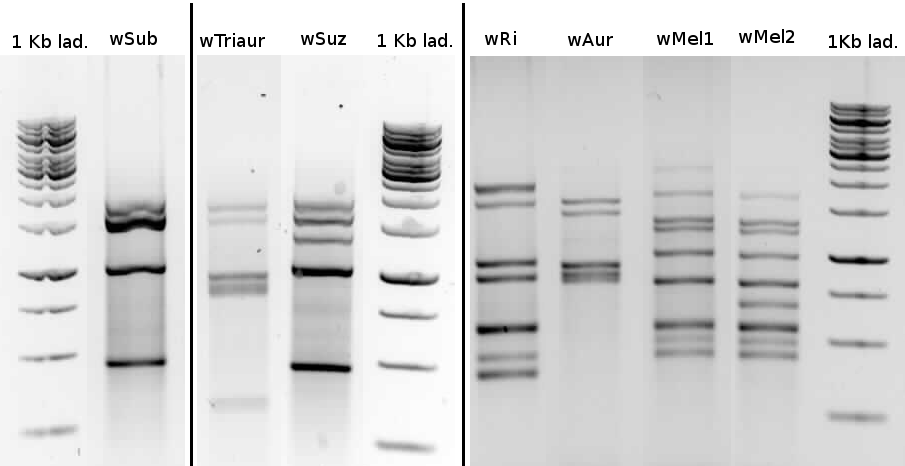
\includegraphics[width=150mm]{images/profils_crop.png}
	\end{center}
	\caption{Reconstruction d'un gel représentant tous les profils carractéristiques des souches de \esp{Wolbachia} en transposon-display avec les amorces Isb/LNP.}
	\label{fig:profils}
\end{figure}

% paragraph polymorphisme (end)

\paragraph{Une amélioration nette du protocole.} % (fold)
\label{par:proto}
Un des éléments notables dans les gels d'éléctrophorèse obtenus est la nette amélioration de l'amplification des fragments de grande taille, notamment pour les profils de type \textit{wMel} (Cf. Figure \ref{fig:wMelcomp}). 
\begin{figure}[tb]
	\begin{center}
		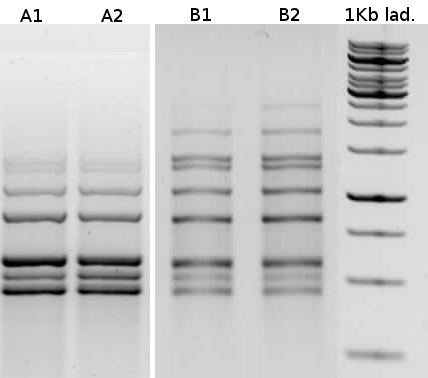
\includegraphics[width=80mm]{images/wMel_comp.png}
	\end{center}
	\caption{Comparaison des deux protocoles sur wMel (\esp{Wolbachia} de \esp{D. melanogaster})~:
	A1 et A2 : Ancien protocole\cite{memHH}~;
	B1 et B2 : Nouveau protocole, avec accuTaq}
	\label{fig:wMelcomp}
\end{figure}
% paragraph proto (end)

% section r_sultats (end)

\section{Conclusion \& Perspectives} % (fold)
\label{sec:ccl}
Afin de tirer des conclusions complètes sur les tranferts horizontaux, il faut encore attendre les résultats de transposon-display sur des lignées de \esp{L. heterotoma} infectées par une seule souche de \esp{Wolbachia}.
Nous ne possédons pas encore ces lignées, mais une seconde partie de ce stage, non développée ici; a consisté à démarrer un traitement antibiotique ménagé sur des \esp{L. heterotoma} tri-infectées (statut d'infection sauvage), afin d'obtenir des lignées présentant un statut d'infection différent pour enfin les typer en transposon-display.

La suite de ce travail consistera à séquencer les fragments obtenus afin de situer précisément les insertions dans le génome, afin d’éventuellement en tirer des conclusions sur les conséquences physiologiques des différentes insertions du transposon. Peut-être trouverons-nous là une piste pour expliquer l’adaptabilité exceptionnelle de \esp{Wolbachia} aux changements d’hôtes ?
% section conclusion_&_perspectives (end)


\printbibliography

\newpage
\pagestyle{empty}
\renewcommand{\baselinestretch}{1} % Pour enlever l'interligne 1.5
\begin{abstract}
Ceci est un résumé qu'il est trop bien.

À imprimer à part, pour l'intégrer à la quatrième de couverture.

Peut-être le compiler à part, dans un autre fichier. On verra.
\end{abstract}
\end{document}
